\documentclass[../thesis/thesis.tex]{subfiles}
\renewcommand{\baselinestretch}{1.5}\selectfont
\graphicspath{{../figs/ch2-rfmwmeas/}}

\begin{document}
\begin{refsection}
\setcounter{chapter}{1}
\chapter{Radio Frequency and Microwave \\Measurements}
\section{Introduction}

To characterise nonlinear behavioural models, the radio frequency (RF) response of a device to electromagnetic wave stimuli must be measured. When compared with DC (and low frequency) measurements, RF and microwave measurements present significant additional challenges. 
For DC systems, it is desirable to propagate voltages through a circuit with minimal loss in amplitude. To achieve this effectively, components are typically designed with high input impedance and low output impedance. With RF systems, circuit components and interconnects can be of the order of a quarter-wavelength in length, and therefore signals must be treated as electromagnetic waves to account for different behaviour at these frequencies.
When a travelling wave encounters a discontinuity in impedance, such as a cable connector or on-wafer structure, some of the power in the wave is reflected. The amount of reflected power is proportional to the size of the impedance mismatch between each side of the discontinuity. Hence, for RF systems, the transmission of power is the focus of the circuit designer. The measurement of power flowing through a transmission line is complicated by three key factors. Firstly, because the waves are travelling, the instantaneous voltage at any point on the transmission line will vary between the peak-to-peak values of the wave. Secondly, there are waves travelling in both directions along the transmission line which must be measured separately. Finally, the power of the wave is a complex quantity which consists of both magnitude and phase.
To perform these measurements, a specialist instrument called a vector network analyser (VNA) can be used. In this chapter, the concepts and measurements associated with this instrument are introduced, which will be used later in the thesis to understand the uncertainty contributions from measurements to nonlinear behavioural models.

\section{Electromagnetic Wave Parameters}
\subsection{Wave Definitions}

To describe the power of electromagnetic waves propagated through a transmission line, several definitions are in use in industry and academia for either accuracy or convenience. To avoid confusion in this document, these will now be defined. Information presented in this section has been obtained from [1-5].

\subsubsection{Travelling Waves}

Travelling waves represent a solution to Maxwell's equations along a transmission line. They are physical and measurable via slotted line experiments or thru-reflect-line calibrations [6] (see Chapter X). Travelling waves are defined by the total transverse electric and magnetic fields $\bm{E}_\textrm{t}$ and $\bm{H}_\textrm{t}$ of a single propagating mode at each frequency:
\begin{equation}
\bm{E}_\textrm{t}=c^+e^{-\gamma z}\bm{e}_\textrm{t}+c^-e^{+\gamma z}\bm{e}_\textrm{t},\quad
\bm{H}_\textrm{t}=c^+e^{-\gamma z}\bm{h}_\textrm{t}-c^-e^{+\gamma z}\bm{h}_\textrm{t}
\end{equation}
where, following the notation of [5], $\bm{e}_\textrm{t}$ and $\bm{h}_\textrm{t}$ are the un-normalized electric and magnetic fields of the modal solution of Maxwell’s equations in transmission line, $\gamma=a+ib$ is the complex propagation constant of the mode, $z$ is the direction of propagation, and $c^+$ and $c^-$ are complex quantities representing the un-normalized forward and backward amplitude of the mode, respectively.

\subsubsection{Equivalent-Circuit Voltage and Current}

To represent travelling waves as equivalent low frequency circuit parameters such as voltage and current, a normalisation is chosen to derive a characteristic impedance for the transmission line. This normalisation takes the form
\begin{equation}
\bm{E}_\textrm{t}(z)=\dfrac{v(z)}{v_0}\bm{e}_\textrm{t},\quad
\bm{H}_\textrm{t}(z)=\dfrac{i(z)}{i_0}\bm{h}_\textrm{t},
\end{equation}
where $v_0$ and $i_0$ are normalisation constants that allow $v$ and $i$ to take units of root-mean-square voltage and current, respectively [5].

\subsubsection{Pseudowaves}

Equivalent voltages and currents cannot be used in lossy transmission lines where the electric and magnetic fields are out of phase. To account for this and provide a solution which can be used with conventional circuit design methodologies (e.g. Smith chart techniques [7]) and simulators, pseudowaves can be used. This representation is defined with a reference impedance, $Z_\textrm{ref}$, which can be chosen by the user, but is typically 50-$\Omega$ in conventional measurements. The forward and backward pseudowaves $a$ and $b$ can be written as:
\begin{equation}
a(Z_\textrm{ref})=\bigg[\dfrac{|v_0|}{v_0}\dfrac{\sqrt{\Re(Z_\textrm{ref})}}{2|Z_\textrm{ref}|}\bigg](v+iZ_\textrm{ref}),\quad b(Z_\textrm{ref})=\bigg[\dfrac{|v_0|}{v_0}\dfrac{\sqrt{\Re(Z_\textrm{ref})}}{2|Z_\textrm{ref}|}\bigg](v-iZ_\textrm{ref})
\end{equation}

\subsubsection{Power Waves}

Finally, power waves are defined so that the relationship $P = |a|^2 - |b|^2$ is true for any reference impedance, where $P$ is the power transmitted through the transmission line and $a$ and $b$ are the forward and backward power waves, respectively. They are defined as:
\begin{equation}
a(Z_\textrm{ref})=\dfrac{v+iZ}{2\sqrt{\Re(Z_\textrm{ref})}},\quad b(Z_\textrm{ref})=\dfrac{v-iZ}{2\sqrt{\Re(Z_\textrm{ref})}}.
\end{equation}
Data taken from Keysight instruments used later in this work is presented in power wave format, with units of square-root Watts. To convert these values into decibels referenced to 1 milliwatt, the following formula is used:
\begin{equation}
P(\textrm{dBm}) = 10\log_{10}(P(\sqrt{W})^2) + 30
\end{equation}

\subsection{Derived Metrics and Figures of Merit}

The behaviour of a linear microwave device can be completely defined by the complex ratio of electromagnetic waves which are scattered at each port to those which are incident at each port. The combination of these ratios constitutes the scattering parameters (s-parameters) of a microwave device and are used extensively in the design and measurement of microwave systems[ref]. The formal definitions of the s-parameters for a two-port device are
\begin{equation}
S_{11}=\dfrac{b_1}{a_1}\bigg\rvert_{a_2=0},\quad
S_{12}=\dfrac{b_1}{a_2}\bigg\rvert_{a_1=0},\quad
S_{21}=\dfrac{b_2}{a_1}\bigg\rvert_{a_2=0},\quad
S_{22}=\dfrac{b_2}{a_2}\bigg\rvert_{a_1=0},
\end{equation}
where both a and b can be expressed in either pseudowave or power wave representation. The term “scattered” can be interchanged with “transmitted” and “reflected” depending on if the scattered wave is output on a different port, or the same port, to the incident wave, respectively. A signal flow diagram is provided in Fig. 1 showing the relationship between equivalent-circuit voltage and current, pseudowaves/power waves and s-parameters for a two-port device.
The s-parameters of all microwave devices will exhibit some degree of frequency dependence. This effect originates from physical processes occurring in the device and can either be a benefit or hinderance to a design. Most passive components (including cables) will have a usable bandwidth which is an unwanted limitation, whereas microwave filters are a ubiquitous component where the same fixed bandwidth is the main purpose of the device. To capture this frequency dependence, s-parameters are measured across a frequency range and stored in a table, usually in Touchstone format (see Fig.2). An example of the frequency dependence of a filter is shown in Fig. 3. For a device operating in the linear regime, if multiple stimuli at different frequencies are incident on the device, they will not interact with each other. The scattered waves will have the same frequency components as if the stimulus at each frequency was applied separately. This is called the frequency superposition principle and does not apply to nonlinear operating regimes, which will be discussed later in this chapter.

\begin{figure}
	\centering
	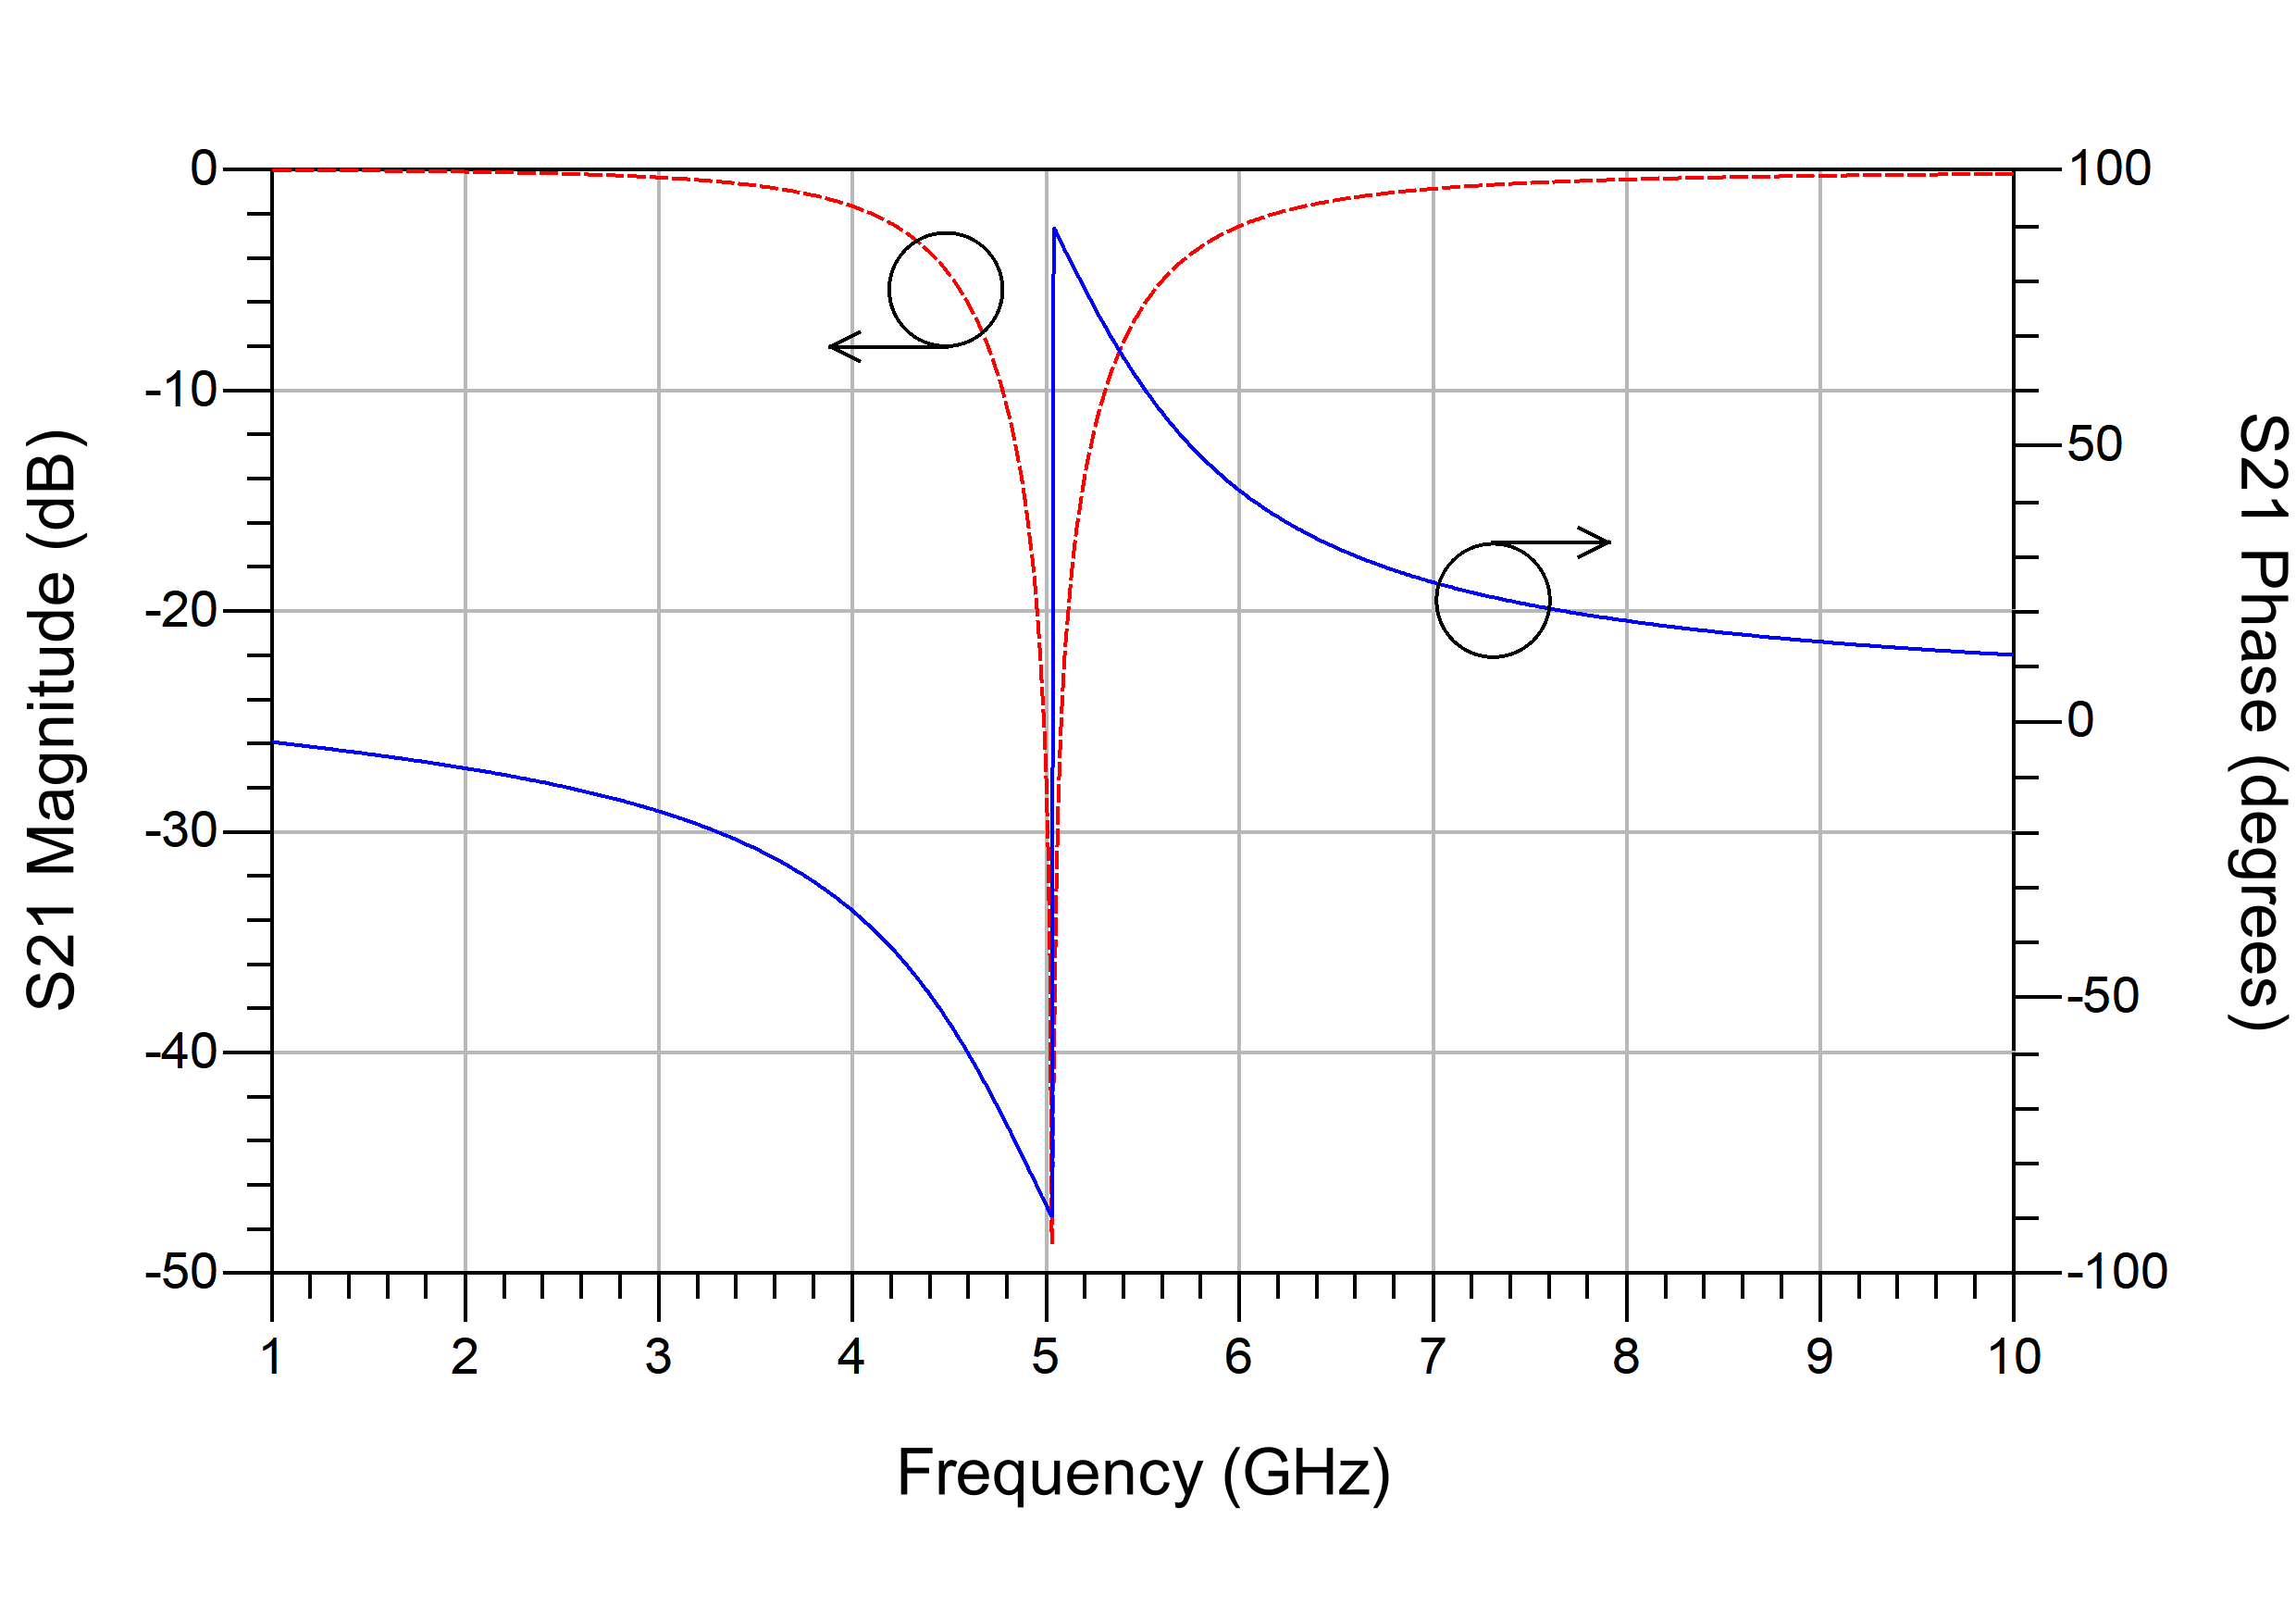
\includegraphics[width=0.8\textwidth]{ch2_filter}
	\caption{The frequency dependence of the magnitude (red dotted trace) and phase (blue solid trace) of $S_{21}$ for a bandstop filter.}
	\label{ch2_filter}
\end{figure}

\begin{figure}
	\centering
	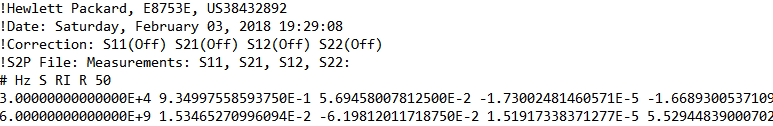
\includegraphics[width=\textwidth]{ch2_s2p}
	\caption{An short example Touchstone file showing a two-port measurement at two frequencies. The rows continue to the right of the figure.}
	\label{ch2_s2p}
\end{figure}

Scattering parameters are often expressed in matrix form, where the column index is the scattered port, and the row index is the incident port. For a two-port device, the s-parameter matrix would be
\begin{equation}
S=
\begin{bmatrix}
S_{11} & S_{12} \\
S_{21} & S_{22}
\end{bmatrix}
\end{equation}

The most interesting characteristic of a two-port microwave device is often the effect which it has on a transmitted wave in the forward direction ($S_{21}$). If the device increases the magnitude of the incident signal this metric is called gain, otherwise it is called insertion loss. Typically gain is associated with active devices (those which are powered from an external source separate to the incident microwave signals) such as amplifiers, and insertion loss is associated with passive devices (those with no external power source) such as attenuators, splitters and mixers. The power gain (operating gain) and insertion loss relating to $S_{21}$ can be calculated using
\begin{equation}
\textrm{Power Gain} = 10 \log_{10} |S_{21}|^2 \textrm{ dB},
\end{equation}
and
\begin{equation}
\textrm{Insertion Loss} = -10 \log_{10} |S_{21}|^2 \textrm{ dB},
\end{equation}
respectively.

Optimal transmission in microwave systems requires impedance matching between components, and it is inevitable that this matching will not be perfect and so some power will be reflected in a two-port device. Therefore, the match of a device is another important measurement, which is dependent on the voltage reflection coefficient ($\Gamma$) of the device and can be related to the impedance of a source and load by
\begin{equation}
\Gamma_{xx} = S_{xx} = \dfrac{Z_\textrm{L}-Z_\textrm{S}}{Z_\textrm{L}+Z_\textrm{S}},
\label{gamma1}
\end{equation}
where $x$ is a port index.
A more thorough definition of voltage reflection coefficient for a two-port device includes any effect from the impedance seen at the other port, and for the case of input match is calculated as
\begin{equation}
\Gamma_{11} = S_{11} + \dfrac{S_{12}S_{21}\Gamma_\textrm{L}}
{1-S_{22}\Gamma_\textrm{L}},
\label{gamma2}
\end{equation}
where $\Gamma_\textrm{L}$ is the voltage reflection coefficient of the load connected to the device. For amplifiers, the amount of isolation (reduction of $S_{12}$) is an important characteristic of the device, whereby a fully isolated amplifier ($S_{12}=0$) is said to be unilateral and equations \ref{gamma1} and \ref{gamma2} are equivalent.

For active devices, such as amplifiers, it can also be useful to consider the power reflected at the input when calculating the power gain of the device. The transducer gain of a device accounts for this potential loss of power at the input and provides a more portable metric which is not dependent on the impedance of the measurement setup. It is defined as
\begin{equation}
G_\textrm{T} = \dfrac{1-|\Gamma_\textrm{S}|^2}
{1-|\Gamma_\textrm{in}\Gamma_\textrm{S}|^2}
|S_{21}|^2
\dfrac{1-|\Gamma_\textrm{L}^2|^2}
{1-|S_{22}\Gamma_\textrm{L}|^2},
\end{equation}
where $\Gamma_\textrm{in}$ is the input match of the device.

For all devices operating in the linear regime, any reflected or transmitted wave will have a frequency equivalent to that incident to the device. In addition, the stimulus power that was used to measure the s-parameters is not important as the ratio of scattered to incident wave magnitude is not dependent on this quantity. However, when microwave devices operate in the nonlinear regime, these conditions no longer apply, and s-parameters cannot be used to capture the full behaviour of the device.

\section{Measurements of Nonlinear Devices}

Microwave devices operating in the nonlinear regime exhibit three differences from their linear counterparts which are significant to the designer:
\begin{enumerate}
\item The amplitude of electromagnetic waves scattered from the device are not linearly dependent on the amplitude of waves incident. This is the cause of features such as gain compression and gain expansion in amplifiers. Some of these effects are solely due to the nonlinear sources inside the device, while others are a symptom of the combined response of the nonlinearity and the power supply. A typical gain compression curve is shown in Fig. 4.

\begin{figure}
	\centering
	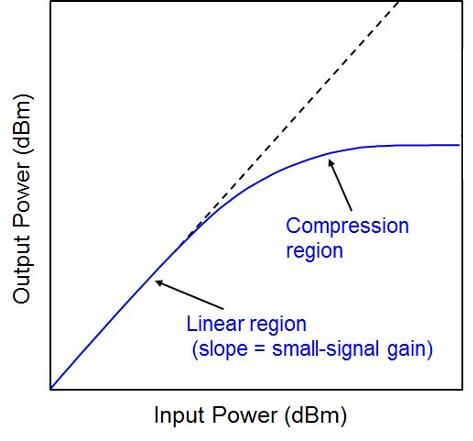
\includegraphics[width=0.4\textwidth]{ch2_comp}
	\caption{Gain compression occurs when an amplifier is driven into a nonlinear operating regime.}
	\label{ch2_comp}
\end{figure}

\item The frequency superposition principle does not apply, and instead the frequency spectrum of scattered waves contains components at frequencies other than those incident upon it. Rather than the incident signals purely summing inside the device, they are also multiplied with each other (frequency mixing), as shown by
\begin{align}
b&=c_0+c_1a+c_2a^2+c_3a^3+\cdots,\\
\alpha=\beta&=2\pi\omega t,\\
a(t)&=A\cos(\alpha),\\
\cos(\alpha)\cos(\beta)&=\dfrac{1}{2}(\cos(\alpha+\beta)+cos(\alpha-\beta)),\\
a^2(t)&=\dfrac{1}{2}A^2[\cos(2\pi(2\omega)t)+1],\\
a^3(t)&=\dfrac{1}{4}A^3[\cos(2\pi(3\omega)t)+3\cos(2\pi\omega t)].
\end{align}
Here, $a$ and $b$ are the incident and scattered waves for the device, $c_i$ are coefficients of the device's nonlinear transfer function, and $a(t)$ is a wave in the time domain with amplitude $A$ and frequency $\omega$. For stimuli with a single frequency ($\alpha$=$\beta$, as above), integer multiples of that frequency will be scattered from the device (harmonics). For stimuli with multiple tones ($\alpha\ne\beta$), additional products from combinations of the incident tone frequencies will be scattered (intermodulation). If the nonlinear device is incident with a fixed bandwidth of frequencies, such as the case for communications signals, then sidebands will be produced around the harmonics of the oscillator frequencies. This effect can be troublesome in practical designs where the unwanted sidebands overlap with the useful microwave bandwidth, distorting the signal. For this reason, it is important for designers to be able to accurately measure and characterise this nonlinear effect. Fig. 5 shows example spectra of these effects.

\begin{figure}
	\centering
	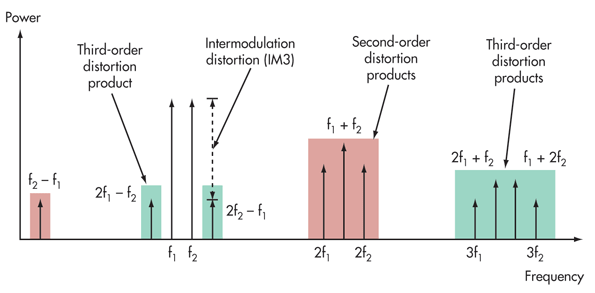
\includegraphics[width=0.8\textwidth]{ch2_im3}
	\caption{Intermodulation products from two tones within the cellular channel bandwidth $f_1$ and $f_2$. The second order products, and upper third order products, can be easily filtered out. However, the lower third order products $2f_1-f_2$ and $2f_2-f_1$ are located within the channel bandwidth and interact with the useful data, increasing EVM and BER \cite{Hall2013}.}
	\label{ch2_im3}
\end{figure}

\item The amplitude of scattered waves with multiple incident waves is dependent (nonlinearly) on the phase of the incident waves. In the linear regime the superposition principle prevents this, but now there is a nonlinear dependence which can have significant effects on the amplitude of scattered waves. Designers must consider this when building efficient nonlinear amplifiers, which leads to the practice of accurately terminating scattered harmonic frequencies at an optimum phase. This will be covered in more detail in chapter X when we discuss nonlinear device models. 
\end{enumerate}
The result of these differences is that the measurement requirements for nonlinear devices are considerably larger than for linear devices. The nonlinear dependencies on stimulus power and phase means that ratioed measurements no longer fully capture the device response, and absolute measurements of the magnitude and phase of both the incident and scattered waves is required. The production of scattered waves at frequencies different to those in the stimulus demands an additional dimension of measurements. In contrast to These complications must be met with changes to both the measurement system and the method of storing the results.

\section{Vector Network Analysers}

To measure the incident and scattered waves for a DUT and calculate the s-parameters as in (5), a vector network analyser (VNA) is typically used. The VNA is a quintessential piece of RF and microwave instrumentation and is found in most if not all such laboratories. Due to the challenging nature of measurements at these frequencies, it is a complicated instrument with many internal parts. This section explains how the VNA functions and the procedures behind its calibration. For a good history of VNA architecture and product development please refer to [Teppati Camb, Dunsmore Wiley].

\subsection{Architecture}

The origin of the VNA lies in an early instrument called a reflectometer. Designed in 1947 by Parzen and Yalow [x], it became an invaluable tool for characterising transmission lines used in telecommunication systems. Shown in Figure x, the incident signal is generated by a swept signal source and passes through the directional coupler before arriving at the DUT. The voltage reflection coefficient of the DUT will cause an amount of incident power to be reflected, which passes back through the coupler before being absorbed by the source (which has very low reflection). The directional couplers allow the waves travelling between the source and the DUT to be sampled by complex receivers, filtering the two waves by their direction of travel thus allowing the incident and scattered waves to be separated for measurement. 

\begin{figure}
	\centering
	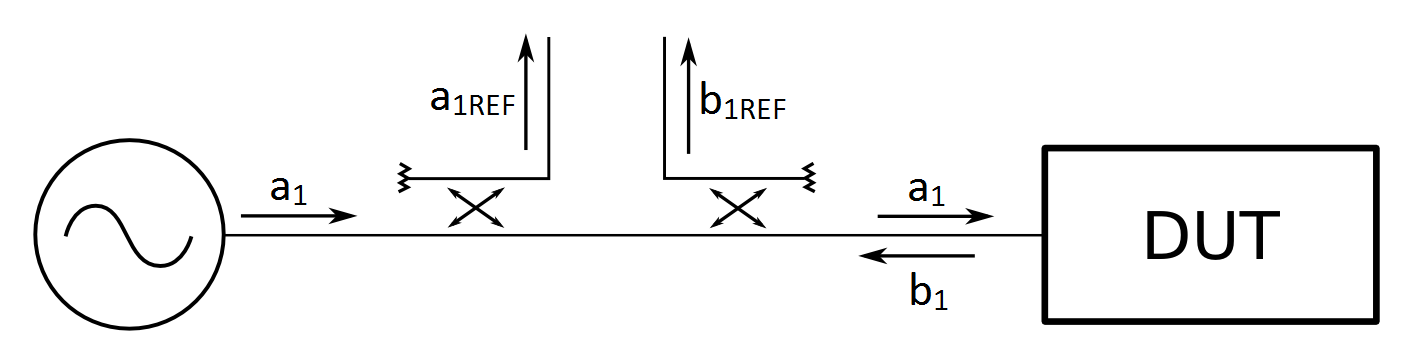
\includegraphics[width=0.8\textwidth]{ch2_refl}
	\caption{A one-port simple reflectometer. $a_1$ is the incident wave generated by the source, which is admitted to the DUT while also being sampled by the directional coupler and sent to the reference receiver via $a_{1REF}$. The reflected wave, $b_1$, is also sampled by another directional coupler and sent to the test receiver as $b_1{REF}$, with the remaining power dissipated at the matched source.}
	\label{ch2_refl}
\end{figure}

The limitation of a single reflectometer is that it can only measure waves at one port of a DUT, therefore preventing transmission measurements. By adding a second reflectometer and synchronising the stimuli and measurements, it is possible to measure all s-parameters of a two-port device. This is the fundamental structure of a VNA, and most variations consist of changing the number of sources or receivers to optimise the instrument for cost or performance. Many older designs use an economical single source which is switched between both ports, whereas now the price of sources has falled, there are instruments available with two independent sources, which allows two-tone and some types of nonlinear measurements. These more versatile units often also expose more  connections between internal components (e.g. the couplers and receivers) to allow the user to perform non-standard measurements or to add attenuation or preamplification for extreme stimulus powers.
Modern VNAs also offer the option of measuring more than two ports, which are referred to as “multi-port” measurements. Several manufacturers offer four-port instruments which include four reflectometers (with usually two sources), although with external switching networks it is possible to expand this up to 48 ports [http://www.microwavejournal.com/articles/21785-vector-network-analysis-with-up-to-48-ports].
The basic block diagram of a modern two-port double-reflectometer VNA is shown in Fig. 9. To measure both stimulus conditions for the two-port S-parameter equations in (5), the sources alternate between delivering power and acting as a load for each measurement. As the source is swept the a and b waves for all ports are measured against frequency, from which the VNA software calculates the S-parameters. The receivers sampling the incident waves are known as the reference receivers and those sampling the scattered waves are called measurement or test receivers.

\begin{figure}
	\centering
	
\includegraphics[width=0.8\textwidth]{ch2_vna}
	\caption{A modern two-source mixer-based VNA, which employs heterodyning to allow measurements at microwave frequencies. Two directional couplers are located between each source and the DUT and are connected back to back. These sample waves travelling in both directions and are connected to mixers which downconvert the microwave frequencies (R) into intermediate frequencies (I) which can be sampled by the complex receivers. The shared local oscillator (LO) feeding the mixers preserves phase coherence between the receivers. This configuration is known as a two-port double-reflectometer VNA. Figure adapted by author from \cite{Root2013}.}
	\label{ch2_vna}
\end{figure}

To perform S-parameter measurements using a VNA, the user must set both the frequency span and number of frequency points. They may also change settings of intermediate frequency bandwidth (IFBW) and numerical averaging, both of which reduce measurement noise by applying digital filtering but can consequently increase acquisition time. The user will then perform a calibration, which corrects for any response present in the measurement setup that is not caused by the DUT. When the system is calibrated physical ‘measurement planes’ are defined, where only effects of the signal path on the DUT side of the planes are incorporated in the measurement results. This is illustrated in Fig. 10. Once this step is complete, the VNA is ready for use. However, it is good practice to first check that calibration was successful by measuring some known devices (verification), or to use techniques such as ripple extraction (discussed in Chapter 4) to measure the residual uncertainty. This process characterises remaining error which the calibration failed to correct.

\subsection{Error Models}

To remove the effect of the measurement setup from the measured device response, an error model is formed to capture the response of the measurement setup during calibration. These error models are stored in the memory of the VNA and are typically de-embedded from the measured device response before the results are presented to the user (although the raw measurements can still be obtained for separate post-processing). Because the measurement setup response is frequency dependent, the error model coefficients are characterised across the measurement bandwidth and are either applied at each measurement frequency or linearly interpolated.

\subsubsection{One-Port Model}

The classic one-port error model can be obtained through analysis of the signal flow diagram of a one-port VNA shown in Fig. 6. One can write the relationship between the measured ($\Gamma_\textrm{M}$) and absolute ($\Gamma_\textrm{A}$) reflection coefficients as
\begin{equation}
\Gamma_\textrm{M}=D+\dfrac{T\Gamma_\textrm{A}}{1-M\Gamma_\textrm{A}},
\end{equation}
where $D$, $M$ and $T$ are error coefficients which capture the unwanted response of the measurement setup. For this model, the three coefficients each have a physical meaning as they are caused by separate physical effects (illustrated in Fig. 7):
\begin{itemize}
\item \textbf{Directivity} ($D$) is caused by the nonideal operation of the directional couplers used to separate the incident and reflected waves inside the VNA. In practice, some amount of incident wave will travel into the test receiver port (vica versa??), reducing the measured gain of the device under test.
\item \textbf{Test port match} ($M$) results from the impedance of the VNA test port (either the original test port or the extended measurement plane including any cables or other components in the setup) being different from the characteristic impedance of the measurement, which is typically 50-$\Omega$. This effect will cause some of the incident wave to be reflected at the test port which is not due to the device response.
\item \textbf{Reflection tracking} ($T$) characterises the insertion loss of the couplers and other measurement components between the reference receiver and the test receiver.
\end{itemize}

\subsubsection{8-Term Model}

Devices with two or more ports require transmission measurements in addition to the reflection measurements which can be corrected using the one-port model. A popular two-port error model, the 8-term model, adds two transmission terms to the method used for the one-port model. This is shown in Fig. blah.

\begin{figure}
	\centering
	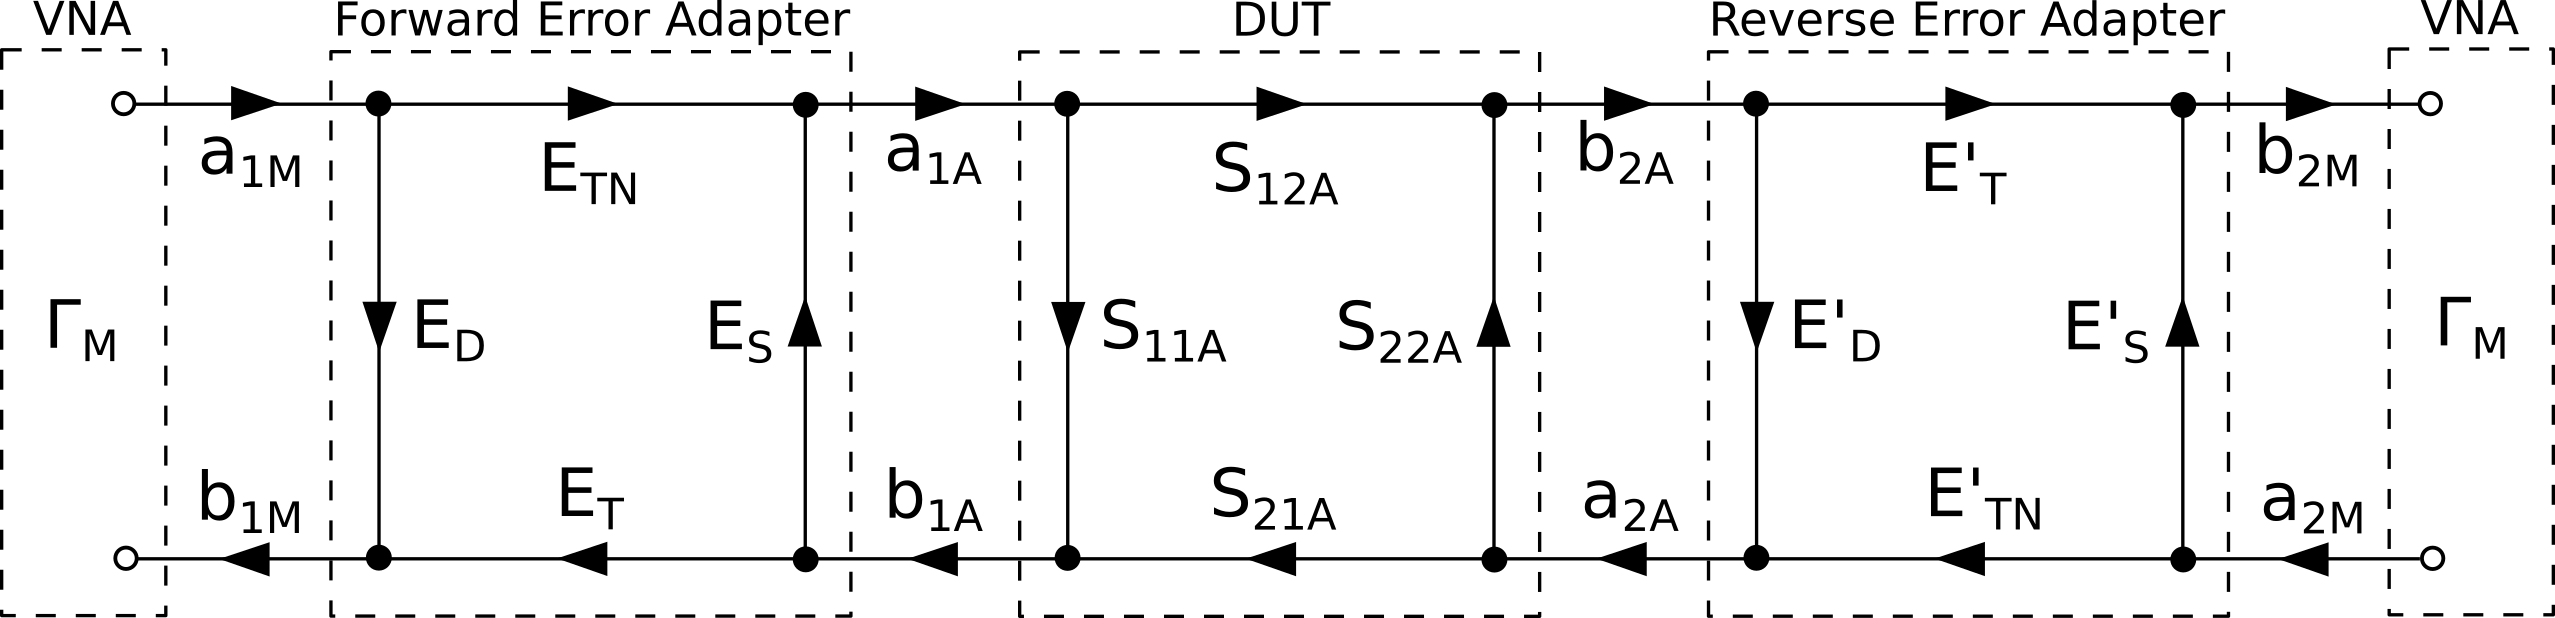
\includegraphics[width=\textwidth]{ch2_8term}
	\caption{The 8-term error model for a two-port measurement. $E_D$, $E_S$, and $E_T$ are the same as for the one-port model, except there are now sets of each for both ports. These extra terms account for different error values when the incident signal is sourced from each port. Additionally for the two-port case, a transmission term $E_{TN}$ has been added for each direction.}
	\label{ch2_8term}
\end{figure}


\subsection{Calibration}
\section{Large Signal Network Analysers}
\subsection{Absolute 8-Term Error Model}
\subsection{Power Meter Calibration}
\subsection{Phase References}
\section{Conclusions}
Testing, testing\cite{Stant_2016_Coll, Stant_2016}.
\addcontentsline{toc}{section}{Bibliography}
\printbibliography
\end{refsection}
\end{document}
